\documentclass[12pt] {article}
\usepackage{times}
\usepackage[margin=0.6in,bottom=1in,top=0.5in]{geometry}

\usepackage{hhline}
\usepackage{subfig}
\usepackage{graphicx}
\usepackage{amsmath}




\begin{document}

\title{Kronecker Product -  EEC289Q}
\author{Ahmed H. Mahmoud}
\date{February 8th, 2018}
\maketitle
%============Table========
%\begin{figure}[tbh]
% \centering    
%\begin{tabular}{ |p{4cm}|| p{2cm}|p{2cm}|p{2cm}|p{2cm}|}
% \hline
% & Processor 1 &  Processor 2  & Processor 3 & Processor 4\\ \hhline{|=|=|=|=|=|}
% \hline
% Performance          &$1.08$        &$1.425$       &\textbf{1.52}  &   \\
% \hline
%\end{tabular} 
%\caption{Metric table for the four processors}
%   \label{tab:metric}
%\end{figure} 
%============Figure========
%\begin{figure}[!tbh]
%\centering        
%   \subfloat {\includegraphics[width=0.65\textwidth]{fig2_4.png}}
%   \caption{ }
%   \label{fig:fig}
%\end{figure}

\paragraph{Analysis.} It is beneficial to start with a little analysis to figure if the problem is compute-bound or memory-bound in order to focus on the right optimization method. At first glance the problem seems memory-bound; for each output value we need to read two values and write one value while only doing one multiply operation. Thus, the arithmetic intensity can not exceed $1/3$. We quantified this by computing the \emph{Speed of Light}; the processing rate that can not be exceeded by assuming that the computation take no time and all memory access are fully coalesced and reside always at the top of the memory hierarchy. In order to carry out the Kronecker product of two matrices $A\in \mathcal{R}^{M\times M}$ and $B\in \mathcal{R}^{N\times N}$ to result into $C\in \mathcal{R}^{\left(M\times M \right)\times \left(N\times N\right)}$, we will need 
$
\underbrace{4M^{2}}_\text{Read $A$} + 
\underbrace{4N^{2}}_\text{Read $B$} +
\underbrace{4(NM)^{2}}_\text{Write $C$}
$
data movement while $(MN)^{2}$ FLOPS are needed. Figure ~\ref{fig:sol} shows the speed of light of different sizes of $A$ and $B$ (see caption) superimposed over the roofline of K40 device. The operation is severely memory-bound and only a very small fraction of peak performance (FLOPS) is achievable.  

\begin{figure}[!tbh]
\centering        
   \subfloat {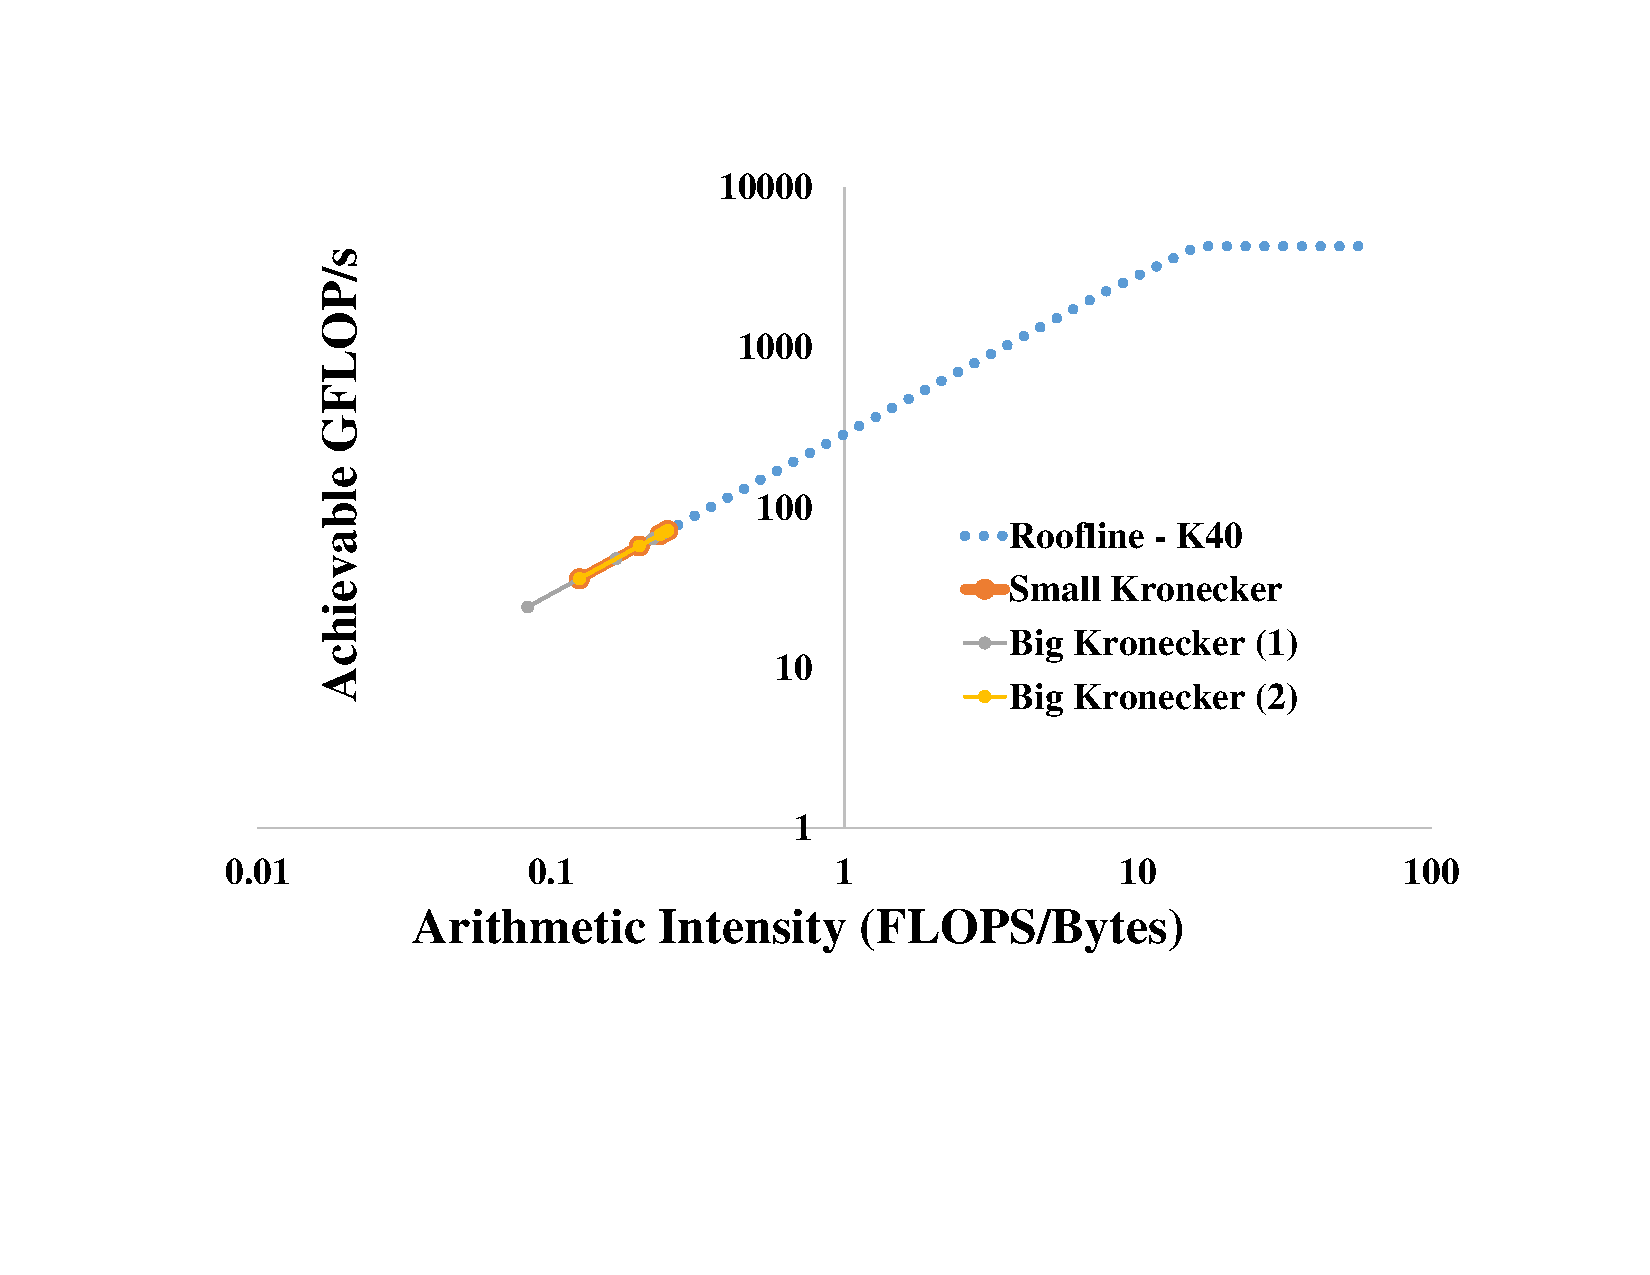
\includegraphics[width=0.5\textwidth]{fig/sol.pdf}}
   \caption{Speed of light of Kronecker product for three different configuration; Small Kronecker is for small $B$ and varying $A$ size, Big Kronecker (1) is for increasing $A$ and $B$ sizes at the same rate, while Big Kronecker (2) starts big $B$ and small $A$ and decreasing $B$ while increasing $A$.}   
   \label{fig:sol}
\end{figure}

\paragraph{Small B.} The main concern here is the memory accessing pattern. An overview of out computation is enumerated below:
\begin{enumerate}
\item each thread will read one and only one value from the input matrix A and shall carry out all the computation assigned for this thread. Given that the maximum size of B is $64 \times 64$, this give a bound on the maximum number of operations done by a thread in one iteration 
\item The whole matrix B shall be present in the shared memory. 
\item Get rid of non-coalesced memory write into C by writing to shared memory first. 
\end{enumerate}

Our computation is carried out by launching number of threads and blocks multiple of the size of A. Each thread reads one entry from A and carries out all the computation needed by this element in A since B is already present in the shared memory. When done, the thread will calculate its stride to read another element of matrix A and do the same. The stride here is $blockDim.x \times gridDim.x$. In order to avoid non-coalesced memory write, we create a scratchpad in a block of size $32\times 32$ (actually it is just 1D array). Each thread will calculate 32 values that will eventually go to C but, instead, write them to shared memory. This is because if each thread write to global memory immediately, all writes will be completely non-coalesced. Figure \ref{fig:c} shows the organization of shared and global memory. In figure \ref{fig:c} (a), if threads writes to global memory instead of shared one, it will be non-coalesced. Figure \ref{fig:c}(b) shows that after writing to shared memory, we carry out the store in global memory in coalesced manner. 


\begin{figure}[!tbh]
\centering        
   \subfloat [Shared Memory] {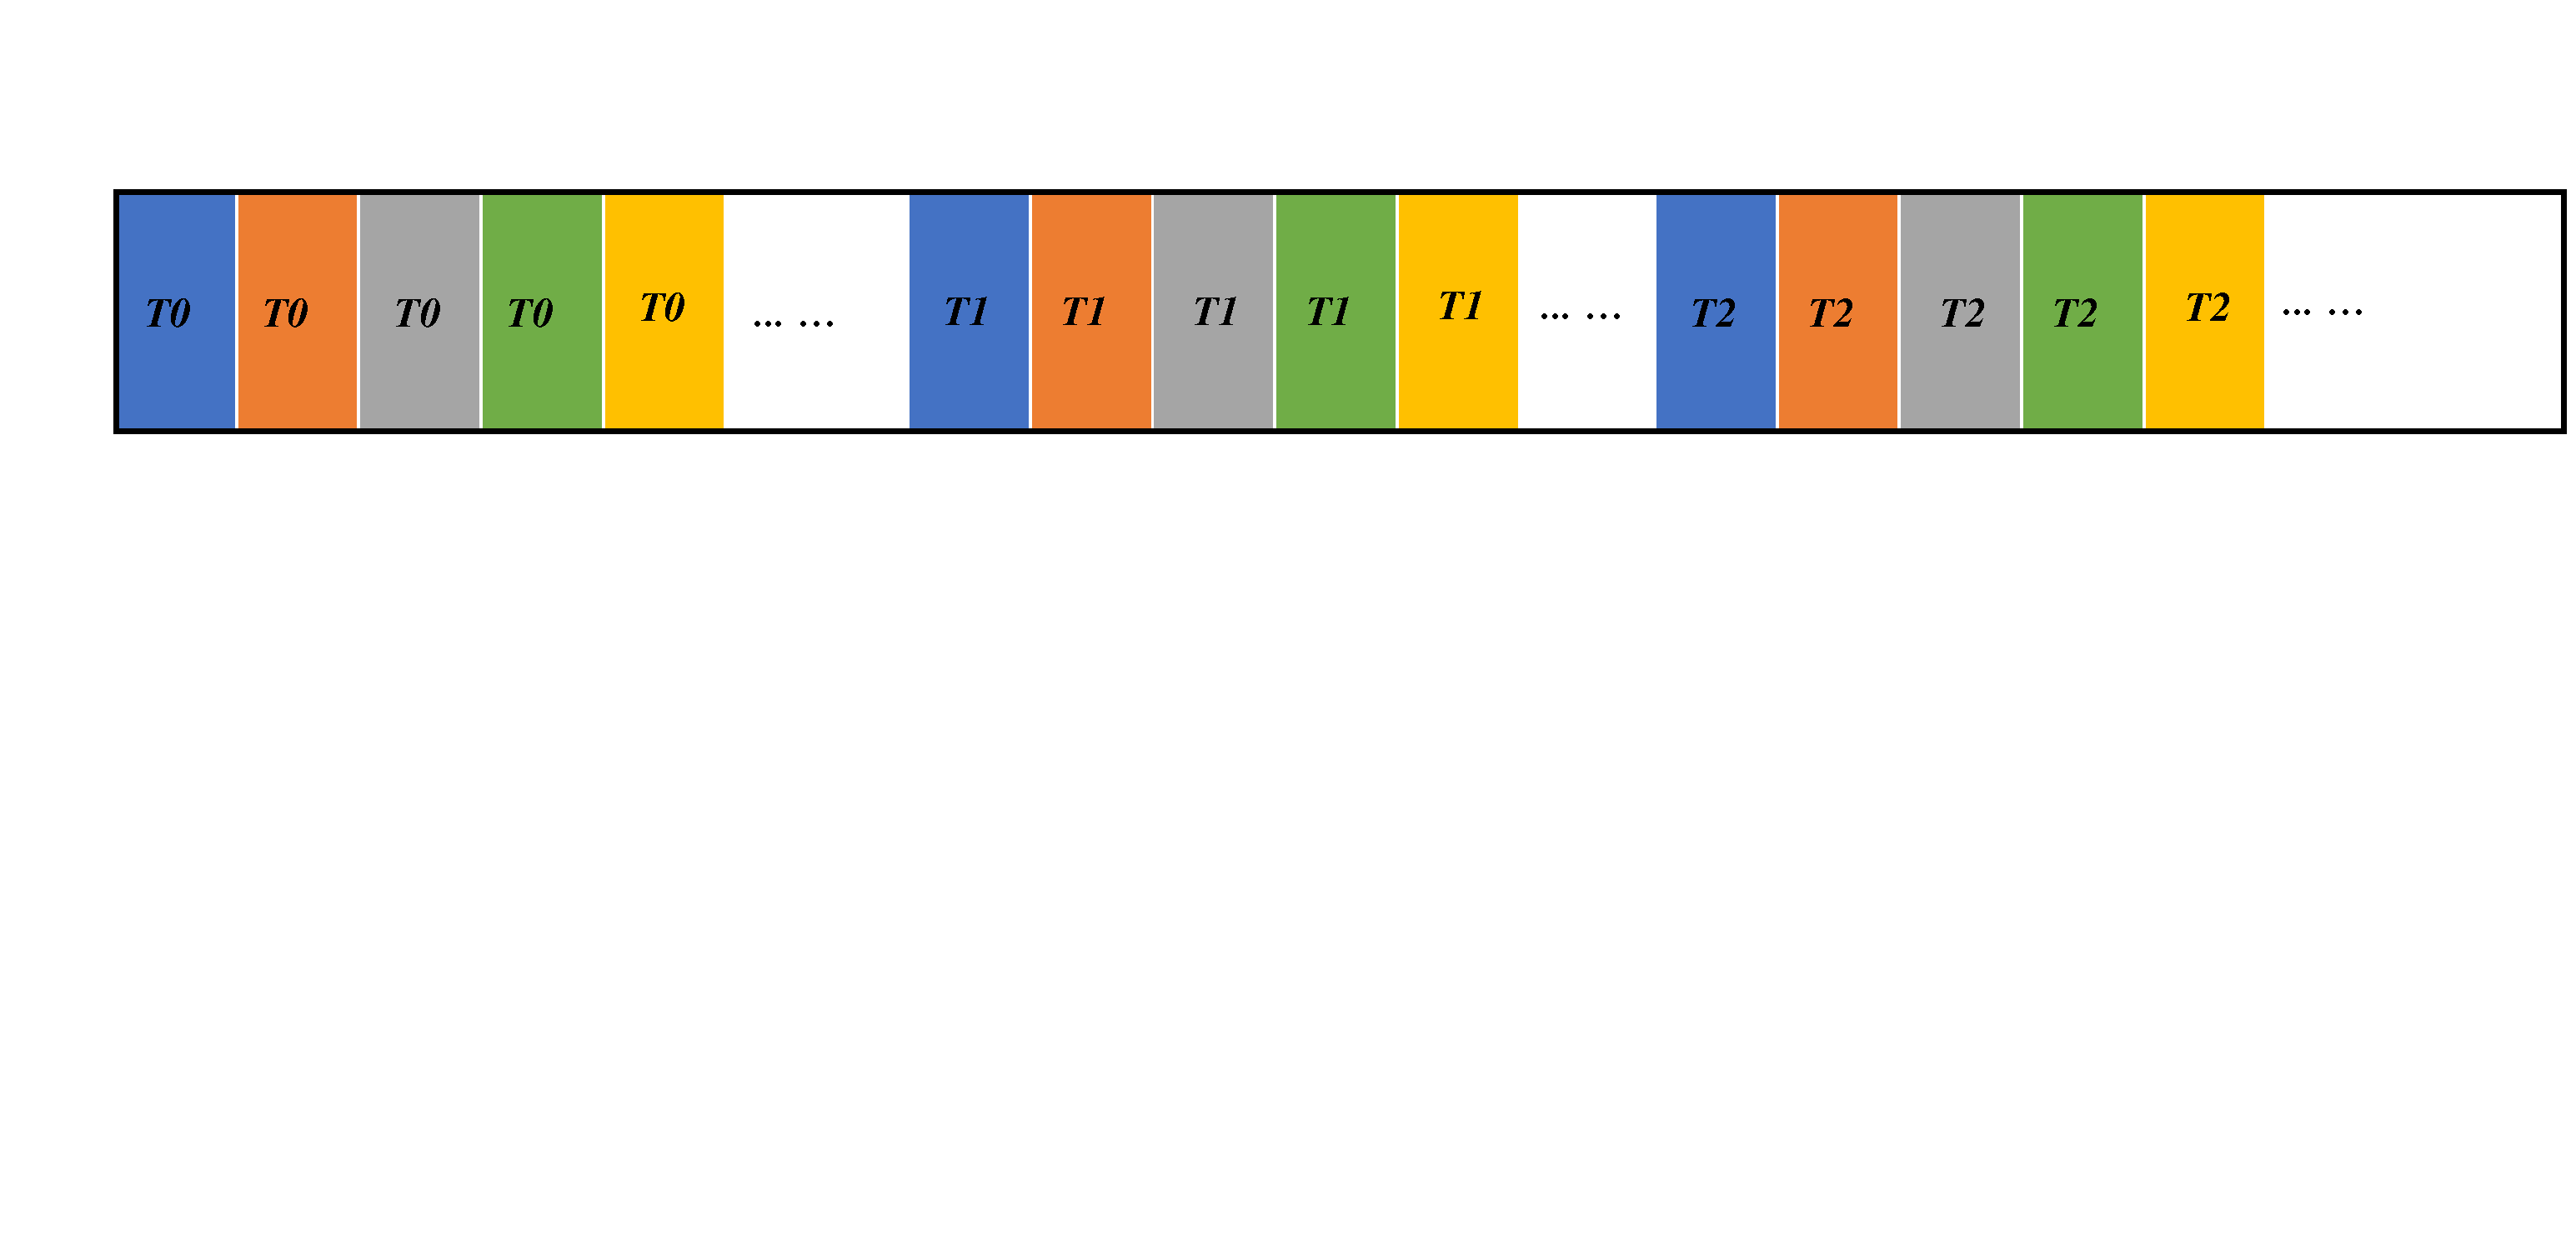
\includegraphics[width=0.6\textwidth]{fig/1.pdf}}
   
   \subfloat [Global Memory] {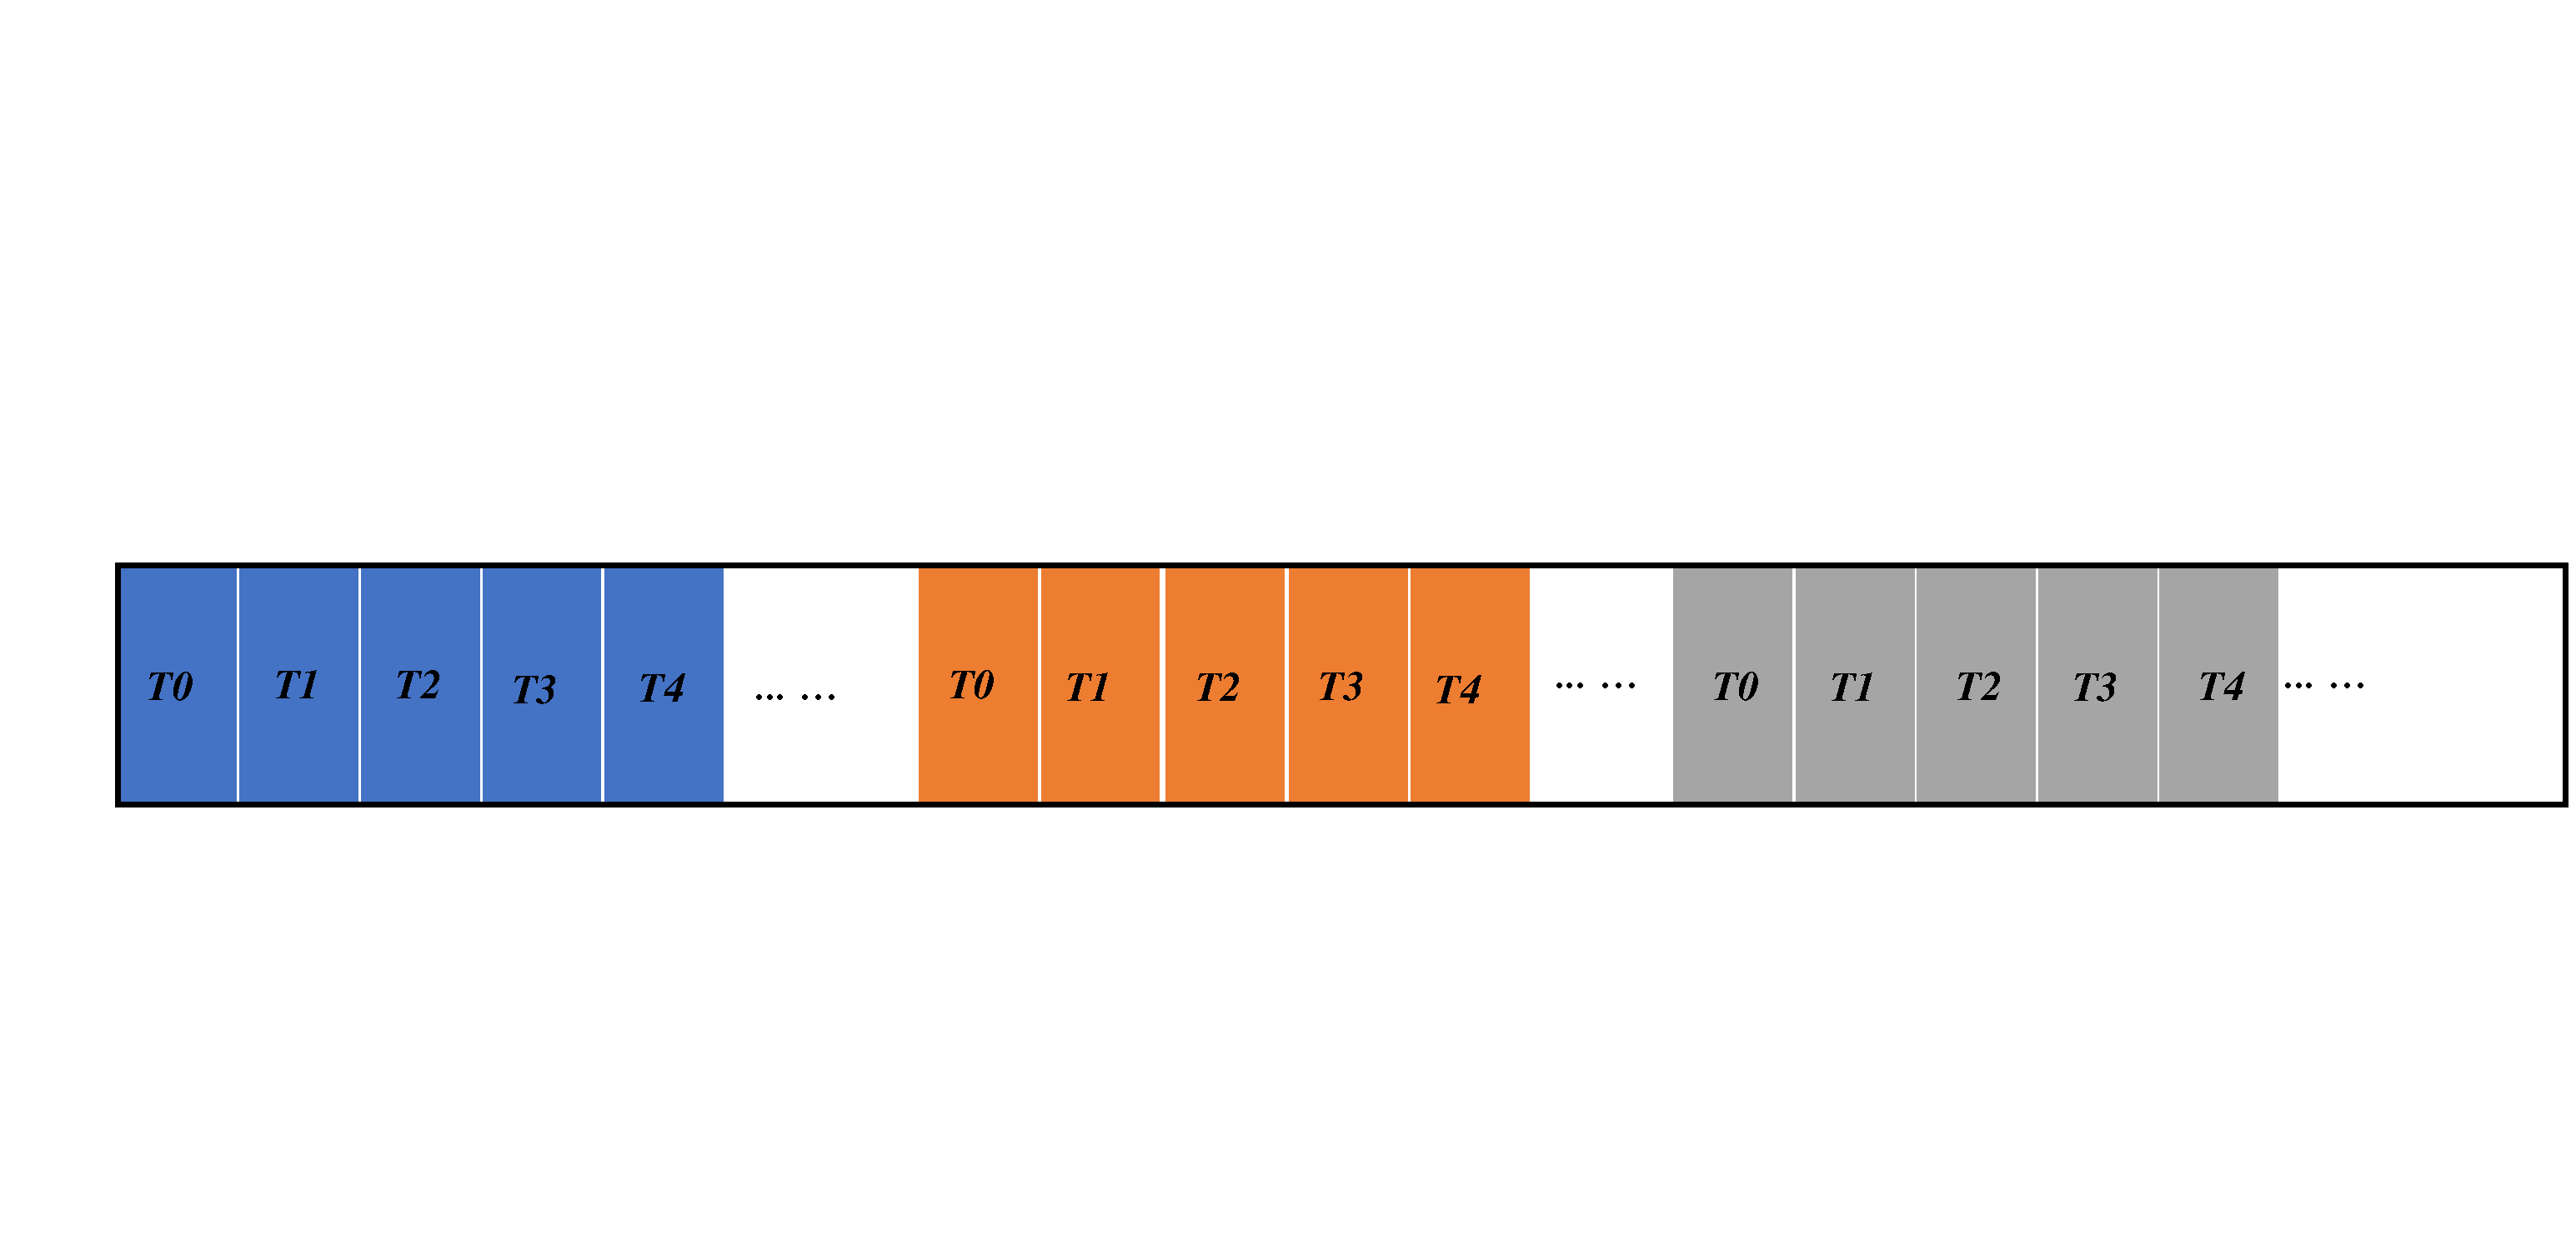
\includegraphics[width=0.6\textwidth]{fig/2.pdf}}
   \caption{Showing the organization of shared and global memory for linearized C matrix and the thread correspondence.}
   \label{fig:c}
\end{figure}

Figure \ref{tab:stat} shows the achieved bandwidth and GFLOPs/Sec using $N = 32$ and 64 with varying values of $M$. After couple of experiments, we found that launching large number of small blocks is more beneficial. For that we fixed the number of threads to be 32 and the blocks to be 512. 

Even though we have get rid of the major bottleneck which is the memory accessing by making sure all read and write are coalesced (verified using the Visual Profiler) and all elements are either read or written just once to the global, the bottleneck has shifted now to be the occupancy. Since we requires $B$ to be present all the time in shared memory and we requires scratchpad in the shared memory, this made the maximum number of warps that can run in parallel between 5 to 2 while the K40 can execute up to 64 warps in parallel.

\begin{figure}[tbh]
 \centering    
\begin{tabular}{ |p{4cm}|| p{2cm}|p{2cm}|p{3cm}|}
 \hline
 & BW($\%$) &  Time (Sec)  & GFLOPs/Sec\\ 
 \hhline{|=||=|=|=|}
 \hline
 M = 32, N=32   & 1.49275  & 0.000930996 &  1.04894 \\
 M = 64, N=32   & 2.03664 & 0.0027275  & 1.43217 \\
 M = 128, N=32  & 2.69394 &0.00824653 & 1.89474 \\
 M = 256, N=32  & 2.74051  &0.0324241  &1.92758 \\
 M = 512, N=32  & 2.75906  &0.128823  &1.94065 \\
 M = 1024, N=32 & 2.76374  &0.514418  &1.94395 \\
 \hhline{|=||=|=|=|}
 M = 32,  N=64  & 0.766877& 0.00724357 & 0.539271 \\
 M = 64,  N=64  & 1.21952 & 0.0182067  & 0.858199 \\
 M = 128, N=64 & 1.35984 & 0.0653001  & 0.957119 \\
 M = 256, N=64 & 1.41011 & 0.251877   & 0.99255  \\
 M = 512, N=64 & 1.41911 & 1.00111    & 0.998892 \\
 
 \hline
\end{tabular} 
\caption{Percentage of bandwidth, time and achieved GFLOPs/Sec for the small B problem.}
   \label{tab:stat}
\end{figure} 



\end{document}
